\subsection*{Question 3.2}

We calculated the eigenvalues and eigenvectors for use in the following subquestions.

\begin{figure}[!htbp]
  \centering
  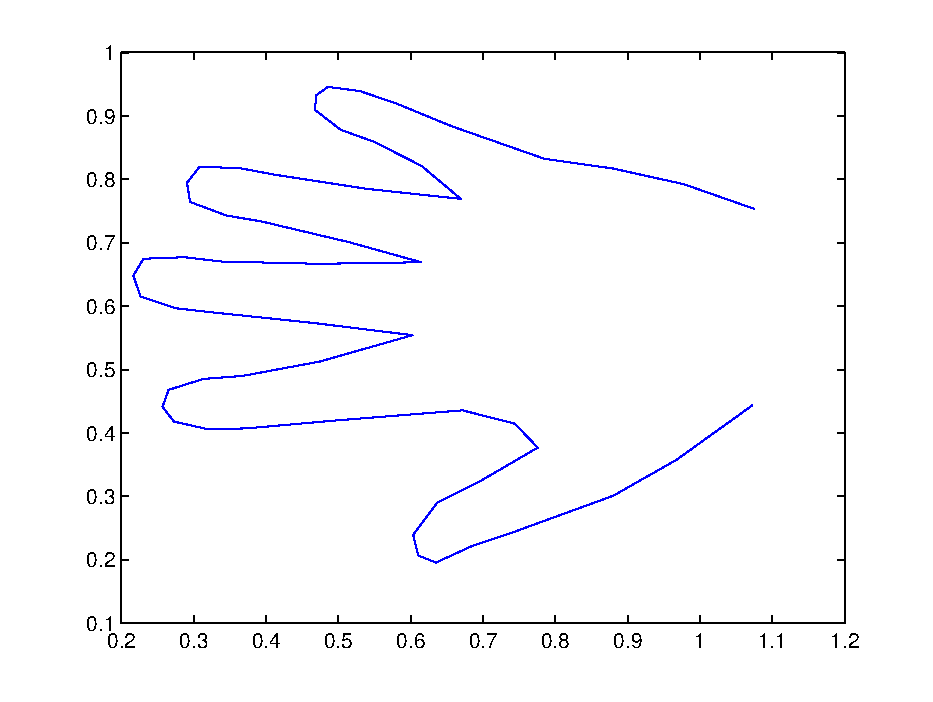
\includegraphics[width=0.85\textwidth]{./images/q32_mean}
  \caption{A hand consisting of the mean value of each data point.}
  \label{fig:q32_mean}
\end{figure}

\begin{itemize}
	\item
	First, we plot the mean values of each point.
	The results can be seen in figure \ref{fig:q32_mean}.
	The hand looks like a normal hand, with no distinct features, so it seems reasonable that this is the average of the hands.
	
	\item
	To visualize the number of components needed to capture the variations, we plotted the accumulated eigenvalues as a function of components used, seen in figure \ref{fig:q32_e}.
	6 components are needed to capture $95\%$ of the variation, and 11 are needed to capture $99\%$.
	Intuitively, it seems that around 5 of the components covers most of the variance, and around 10 covers almost all variation.
	Thus, all components except the first 10 (approximately) can be considered noise.
	
	\begin{figure}[!htbp]
	  \centering
	  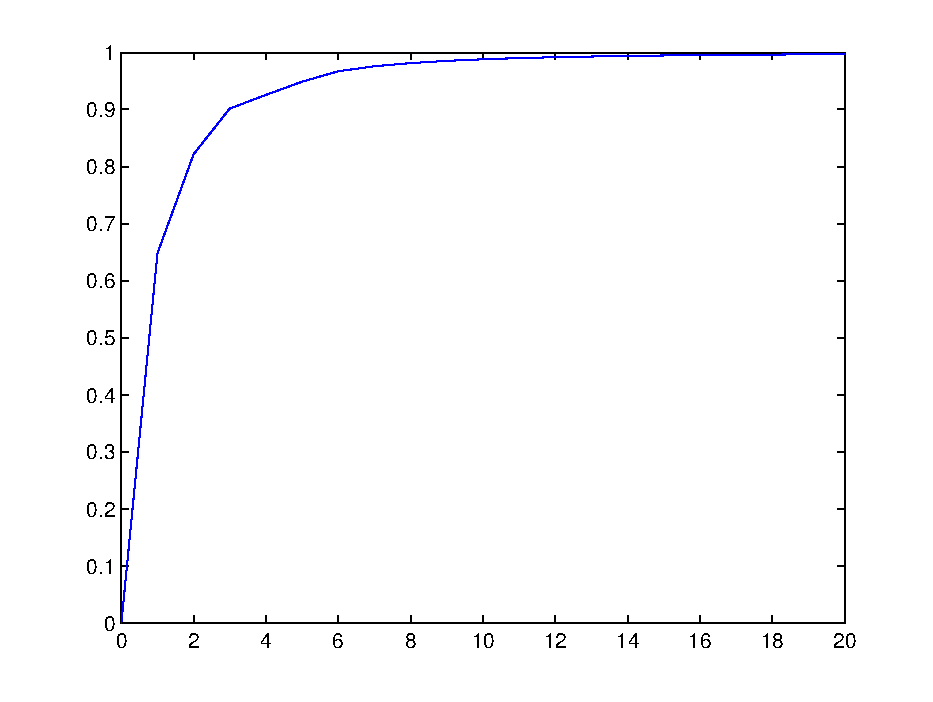
\includegraphics[width=0.85\textwidth]{./images/q32_e}
	  \caption{The amount of variance captured by different amounts of components.}
	  \label{fig:q32_e}
	\end{figure}
	
	\item
	To plot the meaning of the first principal component, we picked the largest eigenvector.
	We normalized the vector and added/subtracted it to/from the mean value (the average hand) to see how it affects it.
	The resulting plot can be seen in figure \ref{fig:q32_c}.
	It looks like the first principal component describes how much the fingers in the hand are spread out.
	This seems reasonable, as it is arguably the most distinct variation between the different hands.
	
	\begin{figure}[!htbp]
	  \centering
	  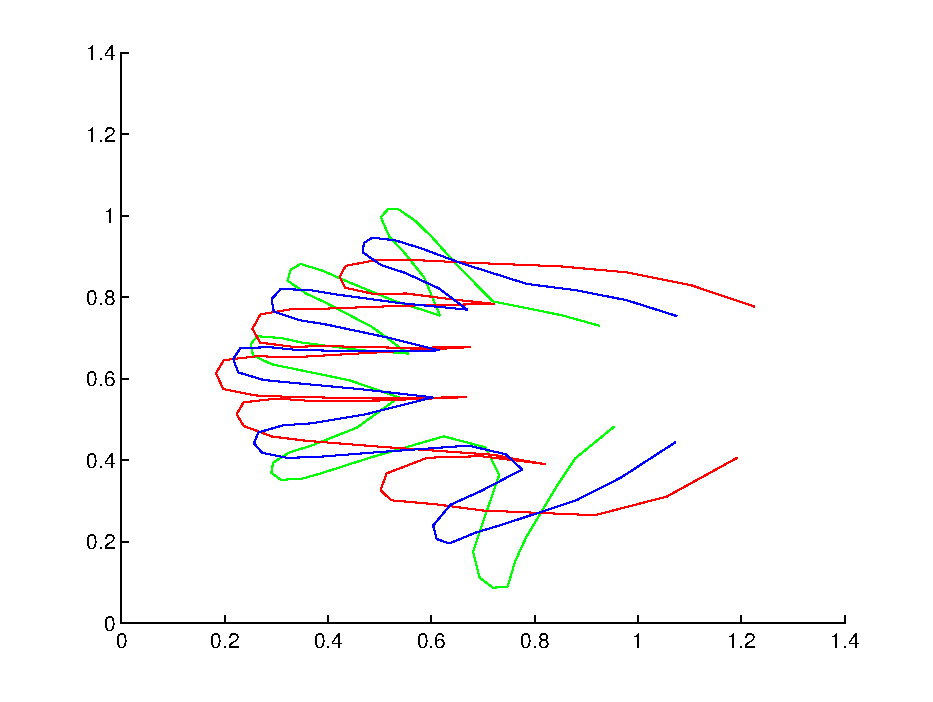
\includegraphics[width=0.85\textwidth]{./images/q32_c}
	  \caption{The mean hand (blue) and the same hand when the first principal component is added (red) and subtracted (green).}
	  \label{fig:q32_c}
	\end{figure}
	
	\item
	This analysis gave us the same kind of information as in question 3.1, but in much greater detail.
	Variating the first principal component shows the same pattern as the covariance plot (where one can see that the fingers can have varying distance to each other), but this analysis concluded how the variations happened together, where the former plot only hinted at it.
	Furthermore, this analysis taught us how many components are needed to describe the variance; a measure that could not be read from the analysis in question 3.1.
	
\end{itemize}
